% !TEX root = thesis.tex
\startfirstchapter{Introduction}
The software industry, often visible through big companies such as Microsoft, Google, IBM, Dell, Apple, Oracle, and SAP, represents several hundred billion dollars of employment and profit a year. 
For example, according to the US Census, the US software industry produced a total revenue of 103.7 billion USD in 2002.\footnote{http://www.census.gov/prod/ec02/ec0251i06.pdf last visited May 10th, 2012}
Similar to many engineering companies, those in the software industry strive to optimize their engineering processes in an attempt to produce higher quality software in a shorter period of time.

Throughout the world, software engineering researchers have dedicated countless hours to improving the manner in which software is developed.
Several fields that are not directly aimed at increasing productivity, such as developing better programming languages~\cite{conf:prog:lang}, smarter compilers~\cite{cong:comp:constr}, and better educational methods to teach algorithms and data structures~\cite{conf:sigcse} contribute indirectly.
Other fields are more directly focused on productivity.
Among them are research in software processes~\cite{conf:icssp}, effort estimation~\cite{molkken:isese:2003,boehm:analse:2000}, and software failure prediction~\cite{conf:promise}.

The vast body of knowledge collected in an attempt to improve the software engineering process is strongly biased towards analyzing the technical side: supporting coding activities (e.g.~\cite{bassil:iwpc:2001,mens:tse:2004}) and analyzing source code to improve quality~\cite{zimmermann:oopsla:2005,nagappan:icse:2006}. 
Since producing source code is the main objective of software developers, optimizing the coding aspect~\cite{bassil:iwpc:2001,mens:tse:2004} as well as analyzing the produced code for issues~\cite{nagappan:icse:2005,schroeter:isese:2006} is important.

Others have focused on the individuals who produce the code. Specifically, studying their behaviour around coding activities~\cite{latoza:icse:2006}, how they communicate~\cite{ko:icse:2007,gopal:2002:comacm}, and how developer relations relate to productivity~\cite{gopal:2002:comacm} and quality~\cite{abreu:iwpse:2009,wolf:icse:2009}.
As in the former case, there is much merit in focusing on the developer.
In the end, the developer implements the features that a software system consists of, and inevitably the developer introduces errors into the code base.

Both studying the human aspect and studying the technical aspect yielded numerous useful results.
For example, on the human side, it appears that the organizational distance between developers is a good predictor of failure on the file level~\cite{nagappan:icse:2008}, and on the technical side similar changes that are timely close are good failure predictors~\cite{kim:icse:2007}.

To truly be able to optimize the software engineering process a more holistic view is needed to bring together both the technical and social aspects.
As stated by Conway~\cite{conway:datamination:1968}, one way to merge these mutually influencing aspects is to use the concept of \emph{socio-technical congruence} in software engineering, which was first formalized by Cataldo et al.~\cite{cataldo:cscw:2006}.
They proposed to overlay networks constructed from social (i.e. who communicates with whom) and technical (i.e. whose code depends on whose source code) dependencies to obtain an overview of a project's social and technical interdependencies and derive insight through the miss-match between the two networks.

%%%%%%%%%%
%%%%%%%%%%
% removed stuff here
%%%%%%%%%%
%%%%%%%%%%


% some of the findings as a teaser
Socio-technical congruence forms a great basis to leverage several digitally recorded data treasures to generate useful and actionable information.
Patterns of developer pairs have shown that when developers share a technical dependency, but are not talking to each other, they are endangering the upcoming software build.
Furthermore, in a student project, we found that certain issues experienced during development can be traced back to code dependencies that could have been detected in real time.

% the two top level research questions
To complement the research that studied the relationship between socio-technical congruence and performance, we focus on \emph{build outcome} as a metric for software quality.
Build outcome is rarely considered when studying software quality, because it is a course measure that often indicates multiple issues rather than a single specific one.
Studying build outcome is important because build success is fundamental in creating a product that can be shipped to a customer.
A successful build towards the end of the release cycle often is the only indicator of customer acceptance with respect to requested features and their stability.
Hence, build success is of utmost importance to a business, as it forms the very product the business hopes to sell.
Therefore, the two guiding research questions we address in this dissertation are:
\begin{description}
\item[RQ 1:] Does Socio-Technical Congruence influence build success?
\item[RQ 2:] Can Socio-Technical Networks be leveraged to generate recommendations to improve build success?
\end{description}

% methodology overview
We are using a mixed methods approach to explore these two research questions.
For \textbf{RQ~1} we employ data mining techniques by studying the artifacts, such as task discussions and source code changes, of a large industrial software project.
\textbf{RQ~2} requires both quantitative and qualitative analysis methods.
To find statistically relevant recommendations we employ data mining techniques, but to explore the usefulness and acceptance of such recommendations we make use of questionnaires, interviews, and observational studies.

\section{Problem Statement}
Socio-technical congruence, as defined by Cataldo et al.~\cite{cataldo:cscw:2006}, describes a measure that outlines the extent by which the technical dependencies in the product are matched by social interactions among developers affected by these technical dependencies.
This directly follows Conway's observations~\cite{conway:datamination:1968}, that the communication structure of any given organization dictates the underlying technical dependencies.
In software engineering, this roughly translates to the idea that the communication flow within software teams needs to match the module dependencies described by the software architecture. 
 
This idea shows great promise when applied to software repositories, such as versioning archives and issue trackers or other recorded communication.
Cataldo et al.~\cite{cataldo:cscw:2006,cataldo:esem:2008}, as well as other researchers~\cite{valetto:msr:2007,ehrlich:stc:2008}, found that the higher the satisfaction of the technical dependencies with social interaction is, the higher the productivity and to some extent the software quality~\cite{kwan:tse:2011,bird:issre:2009,kwan:stc:2009} becomes.
The ability to extract useful socio-technical measures from archives in an automated fashion enables the application to any software project that captures development data electronically.

However, we see three major issues with the concept of socio-technical congruence as it is currently used:
\begin{itemize}
\item The socio-technical congruence measure itself does not give much indication with respect to how to improve the overall situation other than suggesting that people should talk to each other in the event that they share a technical dependency. 
\item The idea of achieving high congruence is based on the notion that it is important to communicate along all technical dependencies, which is not necessarily true.
\item The analysis of socio-technical congruence can only be done post-mortem, which although valuable in a retrospective, does not help to improve productivity or quality in an ongoing project.
\end{itemize}

% item 2
The issue of imbalance between technical and social relationships between developers is related to the problem of not knowing how to improve the socio-technical congruence other than by pointing out the technical relationships between developers that did not communicate with each other.
Given enough resources and time, every technical dependency can be satisfied. 
However, this might run the risk of decreasing the productivity by introducing too many interruptions.

% item 3
Over-communication of technical dependencies might arise from the underlying assumption that every technical dependency warrants the dependent developers to communicate with each other.
We are not solely referring to the ability of  developers to read environment traces~\cite{bolici:stc:2009}, but also to the fact that some changes are either not meant to be communicated or that the system architecture was designed to accommodate certain changes (think of optimizations) that should not affect other developers.

% item 4
To fully leverage the concept of socio-technical congruence it is important to act on it.
The current concept is only shown to relate to performance and quality post-mortem.
To truly unlock the potential of the socio-technical congruence concept it needs to be extended so that it can make on demand recommendations to improve congruence.


\section{Dissertation Focus}
% how do we address the issues
In this dissertation, we focus on addressing the aforementioned issues in two ways:
\begin{description}
% item 3
\item[What technical dependencies need to be met with communication?] 
Although the recommendation to have every developer talk to every other developer about their work seems to be the easiest solution to gaining perfect socio-technical congruence coverage, as previously stated, it could decrease productivity due to the heavy overhead caused by  constant communication.
To address this issue, we seek out which technical dependencies exist among developers and go one step further to try to find the technical dependencies that when not accompanied by communication are the most harmful to the project.

Instead of focusing on recommending changes to the source code to remove technical dependencies we focus on improving the communication among developers.
Because changes to the technical dependencies would partly imply having to re-architect the product, which would be both time intensive and risky, we focus on optimizing the social interactions among developers.
Additionally, as customers rarely derive any tangible benefits from re-architecting a product, there is little willingness to pay for this type of work, unless the re-architecting is the goal as it is the case when porting a legacy system to a new platform~\cite{klinger:mtd:2011}.

% item 4
\item[How to make socio-technical congruence actionable?] Although it is possible that socio-technical congruence can be continuously computed and the previously mentioned strategies can be applied in real time, they all take a more project-centered perspective.
To support developers to engage in communication when necessary, they need to be informed of potential issues that may arise with respect to socio-technical congruence.
Building upon the concept of proximity, proposed by Blincoe et al.~\cite{blincoe:cscw:2012}, we study in depth the development interactions of a large student project at the University of Victoria, Canada, and Aalto University, Finland, and the relation between issues and their fine grained real-time code dependencies.
\end{description}

Furthermore, as Murphy et al.~\cite{murphy:rsse:2010} pointed out, users of automated recommendation systems need to trust the system, otherwise they will ignore it.
This is especially true when continuously reporting information to developers and trying to steer them in a specific direction.
Therefore, we investigate what the daily focus of developers is when it comes to communication to gage if the level of recommendation provided by most methods derived or related to socio-technical congruence might be successful.




\section{Contributions}
This dissertation has two major contributions: (1) an approach to improve social interactions among software developers that leverages the concept of socio-technical congruence and (2)
the findings that coordination, both in terms of structure and absence, negatively influences build success.

\subsection{Approach}
% contribution(s)
The first contribution of this dissertation demonstrates that socio-technical congruence can be used to create recommendations to prevent build failures by improving the social interactions among software developers.
We derived the approach presented in Chapter~\ref{chap:approach} through two case studies that showed that social and socio-technical networks predict build outcome (cf. Chapters~\ref{chap:soc-net} and~\ref{chap:stc-net2}).
In a follow up study, we demonstrate that we could generate relevant recommendations that exhibit a strong influence on build success (cf. Chapter~\ref{chap:soc-net}).
In Chapters~\ref{chap:talk} and~\ref{chap:actionable}, we demonstrated the usefulness of the information with respect to whether experts expect the level of recommendations to be of use, as well as if these recommendations could be produced in real time and potentially prevent issues from arising.
The approach we present in Chapter~\ref{chap:approach} consists of five steps:

\begin{enumerate}
\item Define scope of interest
\item Define outcome metric
\item Build social networks
\item Build technical networks
\item Generate actionable insights
\end{enumerate}

This approach enables us to provide developers with recommendations that point them to engage in communication with other developer they share technical dependencies with.
For example, we found instances where developers, who share a technical dependency but did not communicate, can increase the likelihood of a build failure by more than 80\%.


\subsection{Empirical Findings}
The studies we conducted to motivate and appraise the approach yielded separate research findings extending the body of knowledge of coordination in software development teams. Our approach was inspired by the effect of communication structures on build success that we found with our first study (cf. Chapter~\ref{chap:soc-net}).
Furthermore, we investigated the coordination gaps highlighted by technical dependencies among software developers and their effect on build success (cf. Chapter~\ref{chap:stc-net2}).

In the first study, to the best of our knowledge, we were the first to show a definitive relationship between coordination structures of a development team and build outcome (Chapter~\ref{chap:soc-net}).
We further corroborated this evidence by demonstrating that unmet coordination needs have a negative effect on build outcome as well (cf. Chapter~\ref{chap:stc-net2}).
Then, we presented evidence that specific unmet coordination needs that reoccur over time have a high chance of inducing a build failure (cf. Chapter~\ref{chap:stc-net}).
While investigating whether developers would accept recommendations produced by our approach, we found that the development process influences how concerned developers are about individual changes (cf. Chapter~\ref{chap:talk}).
Finally, in a case study of a large student project at the University of Victoria, Canada, and Aalto University, Finland, we showed that data needed to compute socio-technical network could be collected in real time while a developer edits her source code (cf. Chapter~\ref{chap:actionable}).

\begin{figure}[t]
\centering
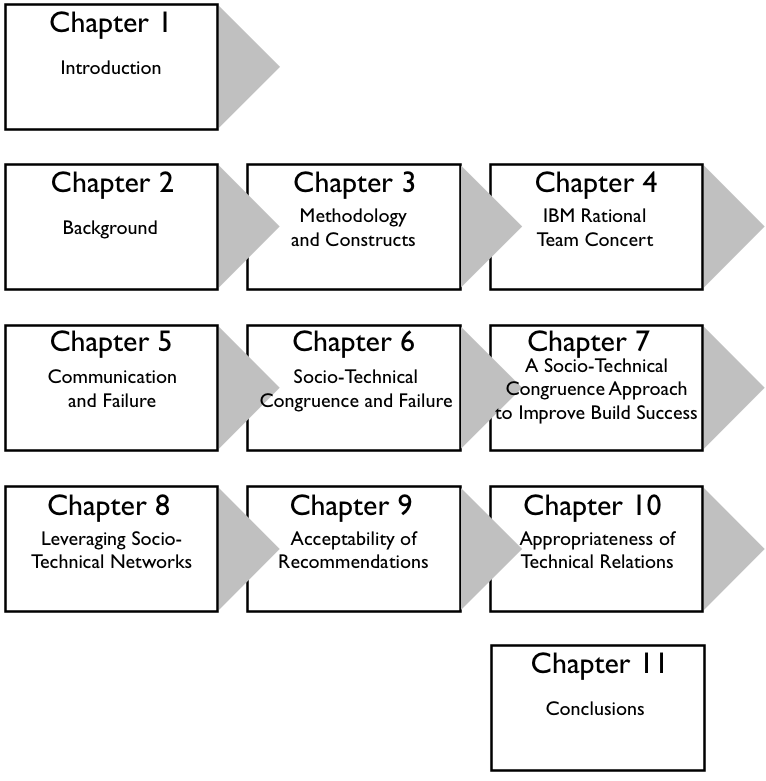
\includegraphics[width=.87\columnwidth]{figures/dis-over}
\caption{Dissertation overview}
\label{fig:over}
\end{figure}

\section{Overview}
This dissertation is divided into three parts (second to fourth row in Figure~\ref{fig:over}).
In part one, we motivate our research by reviewing related work in Chapter~\ref{chap:bg}.
We delve into presenting our overarching methodology with explanations of frequently used constructs and analysis methods in Chapter~\ref{chap:meth}, followed by presenting IBM Rational Team Concert (RTC) as well as some key factors of the development team (cf. Chapter~\ref{chap:rtc}).

Part two presents two studies (cf. Chapters~\ref{chap:soc-net} and~\ref{chap:stc-net2}) that build the foundation for our approach, which we formulate in Chapter~\ref{chap:approach}.
In those two studies, we investigated the relationship between social networks, build success, and socio-technical networks, specifically unmet coordination needs, and build success.

Knowing that the social network might lend itself to manipulations with positive effects with respect to build success, we study the development history of the IBM Rational Team Concert development team for recurring patterns of developer pairs that do not coordinate and their statistical relationship to build success (cf. Chapter~\ref{chap:stc-net}).
We continue by presenting a study in Chapter~\ref{chap:talk}, investigating whether the recommendations resulting from those patterns are of use to developers and when the best time to present such recommendations is.
Before concluding this dissertation we discuss how our approach to leverage socio-technical congruence (cf. Chapter~\ref{chap:disc}) is supported by the evidence uncovered through our studies.
In particular, we present a study in Chapter~\ref{chap:actionable} which provides evidence that our approach can generate recommendations that could have prevented build failures.
Chapter~\ref{chap:disc} outlines the conclusions we derive from our work and points out avenues for future work.




















